\section{Use cases}
\label{sec:use_cases}
The functionality of the system will be defined through use cases, describing how we expect that a user of the system would desire to interact with the system.
The use cases are derived from the requirements described in Section~\ref{sec:problem_domain} and from the use case domain described in the following paragraphs.
The use cases can be seen in Table~\ref{tab:use_cases}.\\


Along with the requirements mentioned in Section~\ref{sec:problem_domain}, a number of assumptions about the usage of \projectname{} form the basis of the use cases in Table~\ref{tab:use_cases}.
These assumptions are our expectations to how the system will be used and therefore how to model it. 
We expect that a number of organization each will have a number of users connected to the system.
At the same time we expect that there will be more users than drones present in the system, and that user-specific permissions to various elements of the system is needed, such as controlling a drone. 

The terms \emph{User}, \emph{Drone} and \emph{Permission} in context of \projectname{} is therefore introduced.
These regulate the relationship between one user in the system and a drone that he wishes to interact with via granted permissions. \\

An example can be an organization that has 10 employees to take care of the security and that this organization has 3 drones in \projectname{}. 
All 10 employees must have access to all 3 drones with user-specific permissions.

We expect multiple users from the same organization to need the same permissions in \projectname{}.
In the case with 10 employees from the organization that needs the same permissions, it may make sense to collect the permissions for the 3 drones in a single Role and assign the 10 users to this role, rather than assigning all permissions for each drone go all 10 users.
Therefore we introduce the terms \emph{Company} to group users and \emph{Rule} to group permissions. \\

These five terms -- user, drone, permission, company \& role -- are the elements that forms the security- and permissions aspect of a users interaction with \projectname{} and that are used in the use cases in Table~\ref{tab:use_cases}.




\begin{figure}[htb]
\begin{center}
\begin{tabular}{ | l | p{12cm} | }
  \hline
	\textbf{ID} & \textbf{User Case} \\ \hline
	%%%%%%%%%%%      %%%%%%%%%%%S
	%%%%%%%%%%% OBS! %%%%%%%%%%%
	%%%%%%%%%%%      %%%%%%%%%%%
	% Inden tallene �ndres, skal der lige gøres opmærksom på det, da de bruges andre steder.
	1 & As a user I want to be able to login into the system.\\ \hline
	2 & As a user, when I am logged in, I want content shown based on my privileges. \\ \hline
	3 & As a user I want to pilot a specific drone.\\ \hline
	4 & As a user I want to view the video feed of a specific drone. \\ \hline
	5 & As a user I want to be able to grant or revoke other users the privileges that I am an admin of. \\ \hline
	6 & As a user with rights I want to change the settings for a specific drone. \\ \hline
	7 & As a user I want to be able to add and remove a drone to a company. \\ \hline
	8 & As a user I want an overview of all drones my privileges grant me access to.\\ \hline
	9 & As a user I want to be able to log out.  \\ \hline
	10 & As a user with rights I want to be able to create and edit users.  \\ \hline
	11 & As a user with rights I want to be able to create a new company.  \\ \hline
	12 & As an owner of a company, I want to be able to edit the company.  \\ \hline
	13 & As a user I want to be able to edit privileges, that I am allowed to edit, for another user.  \\ \hline
	14 & As a user I want to be able to become a customer.  \\ \hline
	15 & As a user I want to be able to add and remove privileges from a role.  \\ \hline
	16 & As a user I want to be able to add roles to users within the company I am allowed to do so.  \\ \hline
	17 & As a user I want to be sure that while piloting a drone nobody else can pilot the same drone. \\
  \hline
\end{tabular}
\caption{Use Cases}
\label{tab:use_cases}
\end{center}
\end{figure}

\clearpage

The use cases define a set of objects which must be present in \projectname{} in order for the use cases to be implementable.
The objects reflect elements in the problem domain which must be modelled in the system.
The objects are \textit{users}, \textit{drones}, \textit{companies}, \textit{roles}, and \textit{privileges}.
This leads to the dependency diagram in Figure~\ref{fig:element_diagram}.
All objects are dependent on privileges, since they either provide or need privileges in order to be used.
Everybody using \projectname{} are classified as \textit{users}, including customers, owners of companies, system administrators etc.
However as reflected in the use cases \textit{users} will not have unrestricted access to the system, as they depend on privileges.
Access to the system will be restricted through \textit{privileges}.
As defined in use case \#8 privileges grants access to functionality, meaning a \textit{user} will not have access to anything by default.
A \textit{drone} refers to a physical drone.
\textit{Companies} is used as a grouping of associated \textit{users}, \textit{drones}, and \textit{roles}.
As an example a company might purchase a set of drones for surveilling their property.
The company would need a set of users for its employees, and a set of privileges granting access to its drones.
The \textit{company} object would handle this grouping.
Use case \#15 defines a role as at set of privileges, that can be associated with a \textit{company} and granted to \textit{users}.
Roles make the process of granting frequently granted privileges easier.
This becomes easier as only one link have to be made to each user, instead of multiple links to multiple users.\\

\begin{figure}[htb]
    \centering
    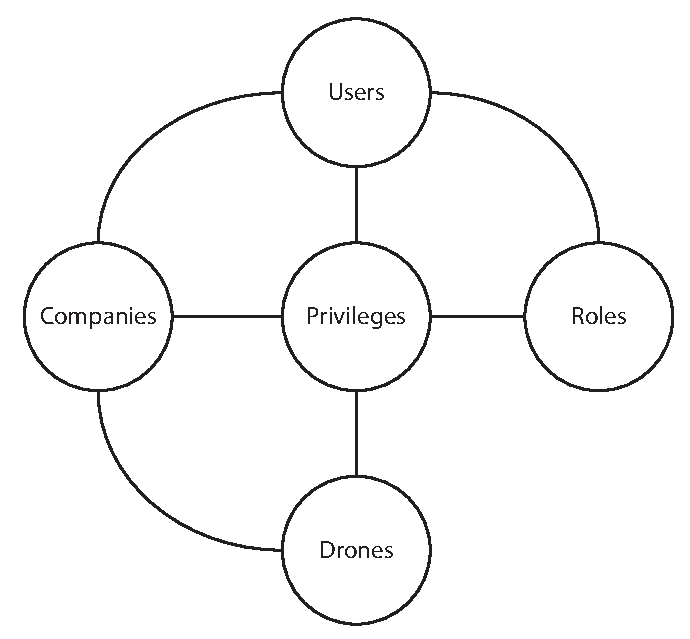
\includegraphics[width=0.95\textwidth]{gfx/element_diagram.pdf}
    \caption{Element Diagram}
    \label{fig:element_diagram}
\end{figure}

As video surveillance is concerned with sensitive information, security in \projectname{} is important.
This is reflected in use case \#1 and \#2.
User authentication is used as the user must login to access to the content of system.
Access is then further restricted with \textit{privileges}, as the user's access to content is based on his privileges.
Privileges must therefore be designed to be applicable to all aspect of \projectname{}, and be able to restrict access to all parts of the system.
Restricting users access to certain parts of the system once they have gained entry is however not sufficient security for such a system.
It must also be considered how the system can be made secure from external attacks.

\clearpage


